% Chapter 1

\chapter{Introduction} % Main chapter title

\label{Chapter1} % For referencing the chapter elsewhere, use \ref{Chapter1} 

%----------------------------------------------------------------------------------------

% Define some commands to keep the formatting separated from the content 
\newcommand{\keyword}[1]{\textbf{#1}}
\newcommand{\tabhead}[1]{\textbf{#1}}
\newcommand{\code}[1]{\texttt{#1}}
\newcommand{\file}[1]{\texttt{\bfseries#1}}
\newcommand{\option}[1]{\texttt{\itshape#1}}

%----------------------------------------------------------------------------------------

\section{Business context} \label{Business context}
This design project is originated from Beenen B.V. in Heerenveen, an industrial automation company that designs and constructs entire control systems for industry, infrastructure and water-technology. With more than 200 employees, divided over the locations Heerenveen, Zwolle and Nijkerk, they execute projects national and international. After delivery, Beenen provide maintenance, support, and inspections to their customers. This maintenance support includes the software inspection and repair of equipment and installations but also services to improve the systems. Currently, this support and service is performed on-site by engineers employed at Beenen Heerenveen or Zwolle. Beenen has customers that construct and deliver installations worldwide with their control systems. Companies in Russia, South-Africa, Brazil and Mexico among others use machines with control systems designed by Beenen. If an installation breaks down and maintenance is required, the needed knowledge to repair is not available on-site in that foreign country. Many installations are able to log and transmit data and therefore it should not be necessary to provide on-site support to maintenance teams. Analyzing data derived from the control systems makes it possible to assist customer maintenance teams worldwide. For this reason, centralizing maintenance at Heerenveen or Zwolle is one of the management goals.

Furthermore, the collected data from customers lend itself for further analysis and processing. For example, an application of predictive maintenance may be possible for customer installations. Predictive maintenance, also called condition-based maintenance (CBM) will be discussed extensively in Section \ref{Literature review}. For now, it can be seen as a tool that can predict upcoming necessary maintenance and therefore reduce unplanned downtime and decreasing total maintenance cost. Beenen tries to decrease the cost of ownership for customers by adding these features to their products. For now, Beenen is not allowed to collect data from customers since the data it is not their property. To be able to provide CBM to their products and services a collaboration with one of their customers, that allows making use of their data, is necessary. The search for a customer that is willing to develop a CBM tool in collaboration with the Research and Development (R\&D) department from Beenen lead to Philips Consumer Lifestyle B.V. in Drachten. Beenen has  established service contracts with Philips Drachten and software engineers are already deployed there. This makes Philips a very useful company to collaborate with in order to obtain production data that can be used by designing a CBM tool. 

Philips Drachten is a developer of numerous innovative products such as shavers, trimmers, vacuum cleaners and coffee machines. The location site at Drachten has 2000 employees, including 600 developers\footnote{https://en.icdrachten.nl/companies/philips}. This project is focused on the maintenance department of the shaver production process. Philips Drachten develops and produces the shaving heads for all Philips shavers, high-end and mid-range shavers. The shaver production department consist of multiple assembly lines (AL), where every line is established to assemble one type of shaver. The shaver ALs are divided over 3 mini-companies called Cypress, Thor and Better-Best, producing the 9000 series, 3000 series and 5000 and 7000 series, respectively. An Support Group, in dutch: Ondersteunende Groep (OG), is assigned to one or more mini-companies and consist of managers and engineers. Members of the Maintenance Technical Support, in dutch: Onderhoud Technische Dienst (OTD), are responsible for the physical maintenance and repair of RACs and other installations at the AL. Functions and corresponding activities of some OG and OTD employees that are of importance for this project can be found in Section \ref{Stakeholder analysis}. Since mini-company Thor features the oldest installations in comparison with the other mini-companies, upcoming maintenance is expected here firstly and this design project will focuses on the ALs at Thor.

To provide guidance to the rest of this thesis, an overview of how the shavers at Philips are produced is given next. All shaver types, mentioned in the previous section, are assembled by multiple robot assembly cells (RAC)s placed in line in large factory halls. RACs consist of robotic arms, tray feeders, vision cameras and specific conveyor belts. The maintenance department, consisting of OTD and OG, is responsible for all maintenance that is necessary for those ALs. Every single shaver is assembled by multiple lines that are divided in the following groups: Hair Chamber Assembly (HCA), Shaver Unit Assembly (SUA), Driving Unit Mechanization (DUM), Basic Body Assembly (BBA), Customization (CUSTO) and Automatic Printed circuit board Process, in dutch: Automatische Printplaat Verwerking (APV). In Figure \ref{fig:assemblyline} it is shown how the different lines are ordered within mini-company Thor. After testing the shavers in the CUSTO, shipment takes place from Drachten to Hungary where the shavers will be packaged and distributed over the global market. All various types of ALs and RACs are not discussed in detail, only the ones that will be focus of this project will be investigated further. However, all mentioned abbreviations will be used often in this thesis and are therefore of importance.
\begin{figure}[ht]
\centering
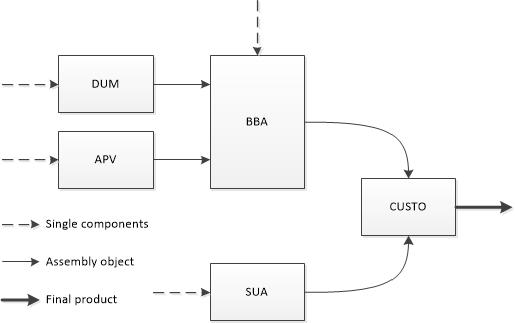
\includegraphics[width=\textwidth]{Figures/assemblyline_Thor}
\caption[Overview of mini-company Thor with corresponding types of ALs]{Overview of mini-company Thor with corresponding types of ALs}
\label{fig:assemblyline}
\end{figure}

\section{Problem context} \label{Problem Context}
Thor's desired production rate is already at a maximum production capacity of 120.000 products per week, which is equal to 1000 products per hour. In comparison, Better-Best and Cypress produce at 70\% and 50\% of their production capacity, respectively. To ensure that an AL is not running out of assembly objects, buffers between every AL are established. The buffer is a storage location, indicated with lines on the floor and info cards, where carts are stored with a maximum capacity of 6. The carts have a capacity of 45 trays, each with 16 place holders, and therefore 720 assembly objects per cart and 4320 per buffer location. The operators of an AL are responsible for placing the carts from the last RAC of an AL, the supplier, to the buffer location and from there to the first RAC of the next AL, the customer, on a First In First Out basis. If maintenance is performed at one AL, the other ALs are continuing  production until the maximum buffer capacity is reached or carts are empty and no assembly objects are available. The last case will result in losses since no assembly objects are arriving at the CUSTO and are finalized. To prevent this from happening, the maintenance department of Philips has the primary task to keep the production running with minimal failures and downtime. Failures can be seen not only as breakdown of equipment but also as other disruptions in the production process. \\
\\
\textbf{(1) Direct Costs:}\\
Labour
\begin{itemize}
\item Normal and overtime labor for
{\setlength\itemindent{15pt} \item planned repair activities}
{\setlength\itemindent{15pt} \item unplanned repairs}
\end{itemize}
Materials
\begin{itemize}
\item Parts replaced
\item Machinery replaced\\
\end{itemize}
\textbf{(2) Indirect Costs:}
\begin{itemize}
\item Lost production (€/hour)
\item Outside services
\item Insurance costs
\item Parts inventory
\end{itemize}
\textbf{Total Potential Cost Reduction (1+2)}\\
\\
\\
\textbf{(3) PdM Program Costs}
\begin{itemize}
\item Site survey
\item Cost of capital equipment
\item Cost of any additional labor
\item Cost of training
\item Initial setup and baseline
\item Scheduled data collection 
\end{itemize}
\textbf{Total PdM costs for one year (3)}\\

Currently, maintenance on the RACs is performed after a breakdown or failure occurs. This type of maintenance is called corrective maintenance (CM) and will be discussed and compared briefly with other maintenance strategies in Section \ref{Literature review}. The RAC will be disassembled and mechanics from the OTD will investigate what the problem is and how to repair it. Depending on the type of maintenance this can be an extensive and time-consuming task. For example, if a harmonic drive of a robot arm is broken, it takes on average 2-4 hours to replace a robotic arm. Since Thor's production rate is already at the maximum, this downtime cannot be overcome and 2000-4000 less products can be produced. This amount of products should be produced in overtime, for example during weekends. As for every company, this overtime is costly and needs to be avoided. Stopping the AL will result in €152,- per hour extra costs.  

Furthermore, an aforementioned harmonic drive has 4 weeks of delivery time and therefore the maintenance department has a few spare parts. This inventory should be kept as low as possible since that the harmonic drives are very costly, €5000,- each. Due to the low amount of spare harmonic drives, a breakdown of multiple harmonic drives around the same time can therefore be catastrophic for the maintenance department of Thor. 

The problem is that there is no efficient maintenance schedule available at Philips and therefore to minimize the inventory and maximize the production rate, one of the maintenance department objectives is to provide an efficient maintenance schedule to their installations. They strive to predict maintenance before failure and adjust the maintenance planning based on that prediction. Similar to the management of Beenen, the maintenance department of Philips has the objective to add CBM to their installations and control systems. 

\section{Research approach} \label{Research approach}
\subsection{Practice oriented research}
Every research or design project aims to provide knowledge, insight and information that can contribute towards solving a problem that can be distinguished into knowledge problems and practical problems \parencite{Verschuren2010}. Where knowledge oriented research (KOR) focuses on knowledge problems by adding knowledge to the knowledge base and practice oriented research (POR) focuses on designing an artifact to solve a practical problem. For this project the problem as described before about the maintenance schedule is of practical nature. To design an artifact, literature have to be reviewed, elaborated and will be used during the design. For this project, no new scientific knowledge will be added to the knowledge base if the maintenance schedule is improved. However, by adding CBM to the RACs and performing experiments new knowledge can be obtained that contributes to the knowledge base. Nevertheless, this project will be considered as POR since obtaining new knowledge is not relevant to the maintenance department of Philips nor the R\&D department of Beenen.

\subsection{The Regulative cycle} \label{The Regulative Cycle}
The regulative cycle is a practice oriented research method that is most useful by design projects. In contradiction, the empirical cycle focuses on knowledge oriented research. The regulative cycle has been applied extensively as a methodology and is formulated by van \citet{vanStrien1986}. It contains the five phases depicted in Figure \ref{fig:Regulative cycle} and described below:
\begin{figure}[ht]
\centering
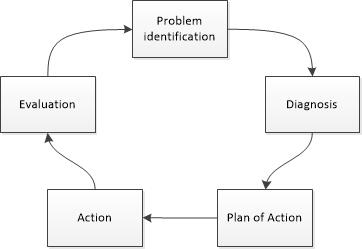
\includegraphics[]{Figures/Regulative_Cycle}
\caption[Regulative cycle]{Regulative cycle based on van Strien \parencite{vanStrien1986,vanStrien1997}}
\label{fig:Regulative cycle}
\end{figure}
\begin{itemize}
\item \textit{Problem identification}; Determines what the exact problem is, why it is a problem and whose problem it is. A specific problem could be defined in order to help with the accurate execution of the research.
\item \textit{Diagnosis}; Examines background and causes of the identified problem. A plan of action can only be formulated if the reason for the problem is understood.
\item \textit{Plan of Action}; Formulates how the problem should be solved by setting up a artifact design.
\item \textit{Action}; Interference of the plan of action formulated in the previous phase. The artifact is applied to the system in order to solve the problem.
\item \textit{Evaluation}; Verifies whether the implemented changes have actually solved the problem. Mostly, the problem is only solved partially and new problems will emerge. The phases described above will then be repeated with the new problems.
\end{itemize}

\subsection{Business System Design} \label{BSD}
The Business System Design (BSD) method, in dutch: OBS method, is a framework formulated by \citet{Prins2008} that describes how to perform the problem identification and diagnosis phases correctly. The diagnosis in BSD is a worked-out approach of the problem identification and diagnosis phase of the regulative cycle. It provides the researcher with a clear guideline throughout these steps of the research. 

The first phase is to address the 'right' problem with corresponding problem owner. This phase is called the problem determining phase and consist of problem owner analysis, system description, stakeholder analysis, problem definition and research goal. After the problem determining phase, the first part of the conceptual research design phase will be addressed where research questions are formulated, literature is reviewed and a conceptual causal model is build. In the second part of the conceptual research design phase, concepts of operationalization, choice of tools and techniques and a data gathering plan are discussed. This problem identification and diagnosis is described in Chapter \ref{Chapter2}. The other phases in the regulative cycle are addressed afterwards. The plan of action that will be executed is constructed in Chapters \ref{Chapter3} and \ref{Chapter4}. The execution will be described in Chapter \ref{Chapter5} and evaluated in Chapter \ref{Chapter6}. A more detailed outline of this thesis will be provide in Section \ref{Thesis outline}